\section{Diskusjon}
\label{sec:diskusjon}

Det finnes flere viktige aspekter rundt informasjonsgjenfinning. Blant annet vil det ofte være naturlig å se på precision kontra recall. Som en del av kursmaterale fikk vi også med en såkalt 'gullstandard' som skulle brukes for å måle ytelsen av søkemotoren som vi har laget.

Precision går på det å se på antall relevante dokumenter av de dokumentene som er valgt. 

Precision = (relevante og hentede dokumenter) / hentede dokumenter. Eks. Om vi har hentet 2 dokumenter, og bare 1 er relevant. Så vil precision være 50\%.

Da ser vi mens recall ser på på antall relevanter dokumenter av totale dokumenter. Recall = (relevante og hentede dokumenter) / (totale dokumenter). Eks. om det finnes 20 dokumenter i kolleksjonen, og 10 av dem er hentet, så vil recall være 50\%. Precision ville vært 100\% i dette tilfelle. 


\paragraph
For å skape et bedre bilde av situasjonen, kalkulerte vi den interpolerte presisjonen for fire recall-nivåer: 25\%, 50\%, 75\% and 100\%.

\begin{tabular}{|m{0.3 \textwidth}|m{0.3 \textwidth}|}
\hline
Recall & $\overline{P}$(r) \\ \hline
25\% & 68\% \\ \hline
50\% & 46\% \\ \hline
75\% & 28\% \\ \hline
100\% & 25\% \\ \hline
\end{tabular}
\captionof{table}{Precision vs Recall}

\begin{center}
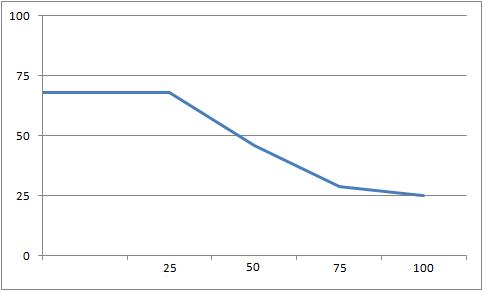
\includegraphics{section/recallgraf}
\captionof{figure}{Precision vs Recall}
\end{center}

Siden Legemiddelhåndboken er et stort dokument som er videre delt i kapitler, subkapitler og subsubkapitler, bestemte vi oss for å kun håndtere kapitler og subkapitler som separate dokumenter. Bakgrunnen for dette var at kapitler og subkapitler har egne HTML-filer i den originale dokumentsamlingen. Det ville vært en mer optimal løsning å dele videre inn i subsubkapitler, for å få resultater med mindre støy. 

Grunnet støy i resultatene fikk vi tidvis dårlig presisjon, spesielt i pasientsak 7 og 8, hvor det ble retunert for mange dokumenter. 

Måten vi delte dokumentene opp på førte også til at vi i enkelte tilfelle fikk totalt feilaktige søk. I pasientsak 5 var ikke 'gold standard'-dokumentet i søkeresultatene i det hele tatt. 

I pasientsak 6 var det forventede dokumentet det høyst rangerte dokumentet. 
I resten av pasientsakene var de forventede dokumentene blant de fem høyest rangerte dokumentene. 



